%%%%%%%%%%%%%%%%%%%%%%%%%%%%%%%%%%%%%%%%%%%%%%%%

% Specify the command that you want into the header of the
% index.md file

%%%%%%%%%%%%%%%%%%%%%%%%%%%%%%%%%%%%%%%%%%%%%%%%

% Options for packages loaded elsewhere
\PassOptionsToPackage{unicode}{hyperref}
\PassOptionsToPackage{hyphens}{url}
\PassOptionsToPackage{dvipsnames,svgnames*,x11names*}{xcolor}
%
\documentclass[
  12pt,
  oneside]{report}
%%\usepackage{lmodern}
%
% Set line spacing
\usepackage{setspace}
\setstretch{1.5}

\usepackage{amssymb,amsmath}
\usepackage{ifxetex,ifluatex}
\ifnum 0\ifxetex 1\fi\ifluatex 1\fi=0 % if pdftex
  \usepackage[T1]{fontenc}
  \usepackage[utf8]{inputenc}
  \usepackage{textcomp} % provide euro and other symbols
\else % if luatex or xetex
  \usepackage{unicode-math}
  \defaultfontfeatures{Scale=MatchLowercase}
  \defaultfontfeatures[\rmfamily]{Ligatures=TeX,Scale=1}
\fi
% Use upquote if available, for straight quotes in verbatim environments
\IfFileExists{upquote.sty}{\usepackage{upquote}}{}
\IfFileExists{microtype.sty}{% use microtype if available
  \usepackage[]{microtype}
  \UseMicrotypeSet[protrusion]{basicmath} % disable protrusion for tt fonts
}{}
\makeatletter
\@ifundefined{KOMAClassName}{% if non-KOMA class
  \IfFileExists{parskip.sty}{%
    \usepackage{parskip}
  }{% else
    \setlength{\parindent}{0pt}
    \setlength{\parskip}{6pt plus 2pt minus 1pt}}
}{% if KOMA class
  \KOMAoptions{parskip=half}}
\makeatother
\usepackage{xcolor}
\IfFileExists{xurl.sty}{\usepackage{xurl}}{} % add URL line breaks if available
\IfFileExists{bookmark.sty}{\usepackage{bookmark}}{\usepackage{hyperref}}
\hypersetup{
  pdfauthor={François Leroy, PhD student at CZU},
  colorlinks=true,
  linkcolor=Blue,
  filecolor=Blue,
  citecolor=Blue,
  urlcolor=Blue,
  pdfcreator={LaTeX via pandoc}}
\urlstyle{same} % disable monospaced font for URLs

%% Package geometry
\usepackage[left = 2cm,right = 2cm,top = 2cm,bottom = 2cm]{geometry}
\usepackage{pdflscape}


%\usepackage{longtable} % out of date, now in latex-tools package
\usepackage{booktabs}
% Correct order of tables after \paragraph or \subparagraph
\usepackage{etoolbox}
\makeatletter
\patchcmd\longtable{\par}{\if@noskipsec\mbox{}\fi\par}{}{}
\makeatother
% Allow footnotes in longtable head/foot
\IfFileExists{footnotehyper.sty}{\usepackage{footnotehyper}}{\usepackage{footnote}}
\makesavenoteenv{longtable}
\setlength{\emergencystretch}{3em} % prevent overfull lines
\providecommand{\tightlist}{%
  \setlength{\itemsep}{0pt}\setlength{\parskip}{0pt}}
\setcounter{secnumdepth}{5}
%%% Complete the preamble of the LaTeX template
%%%------------------------------------------------------------------------------

%% Bug de bookdown: ne traite plus la déclaration "otherlangs" dans le préambule
% Pour charger les langues, écriture ici en dur du produit de bookdown
% Corrigé le 22/11/2019. A retester régulièrement: supprimer ces lignes si la compilation fonctionne sans elles.
\usepackage{polyglossia}
  \setmainlanguage[variant=american]{english}
  \setotherlanguage[]{french}
% Bug persistant le 28/02/2020

% Advised with polyglossia and babel
\usepackage{csquotes}

% Environnement "Essentiel" en début de chapitre
\usepackage[tikz]{bclogo}
\newenvironment{Essentiel}
  {\begin{bclogo}[logo=\bctrombone, noborder=true, couleur=lightgray!50]{L'essentiel}\parindent0pt}
  {\end{bclogo}}

%% Package fontspec
\usepackage{fontspec}
\setmainfont{calibri}[
  Path           = ./fonts/,
  Extension      = .ttf,
  BoldFont       = calibrib,
  ItalicFont     = calibrili,
  BoldItalicFont = calibriz]

% Rename chapters
% Below, scrpit to prevent the "chapter n" and the space use for it to
% be displayed
\usepackage{titlesec}
\titleformat{\chapter}   
{\Huge}{\thechapter{. }}{0pt}{\Huge}
%{\thechapter{. }}
\titlespacing*{\chapter}{0pt}{-50pt}{10pt}
% -50 is to up the title and 10 is the space with the text below


% When using the natbib biblio package, includes "References" in the table of contents
\usepackage[nottoc]{tocbibind}

% To make the table caption full page width
\usepackage{caption}
\usepackage{booktabs}
\usepackage{longtable}
\usepackage{array}
\usepackage{multirow}
\usepackage{wrapfig}
\usepackage{float}
\usepackage{colortbl}
\usepackage{pdflscape}
\usepackage{tabu}
\usepackage{threeparttable}
\usepackage{threeparttablex}
\usepackage[normalem]{ulem}
\usepackage{makecell}
\usepackage{xcolor}
\ifluatex
  \usepackage{selnolig}  % disable illegal ligatures
\fi
\usepackage[]{natbib}
\bibliographystyle{apa}

\author{François Leroy, PhD student at CZU}
\date{2021-09-11}

% to include pdf
\usepackage{pdfpages}



%%%%%%%%%%%%%%%%%%%%%%%%%%%%%%%%%%%%%%%%%%%%%%%%%%%%%%%%%%%%%
% Start of the documents
\begin{document}

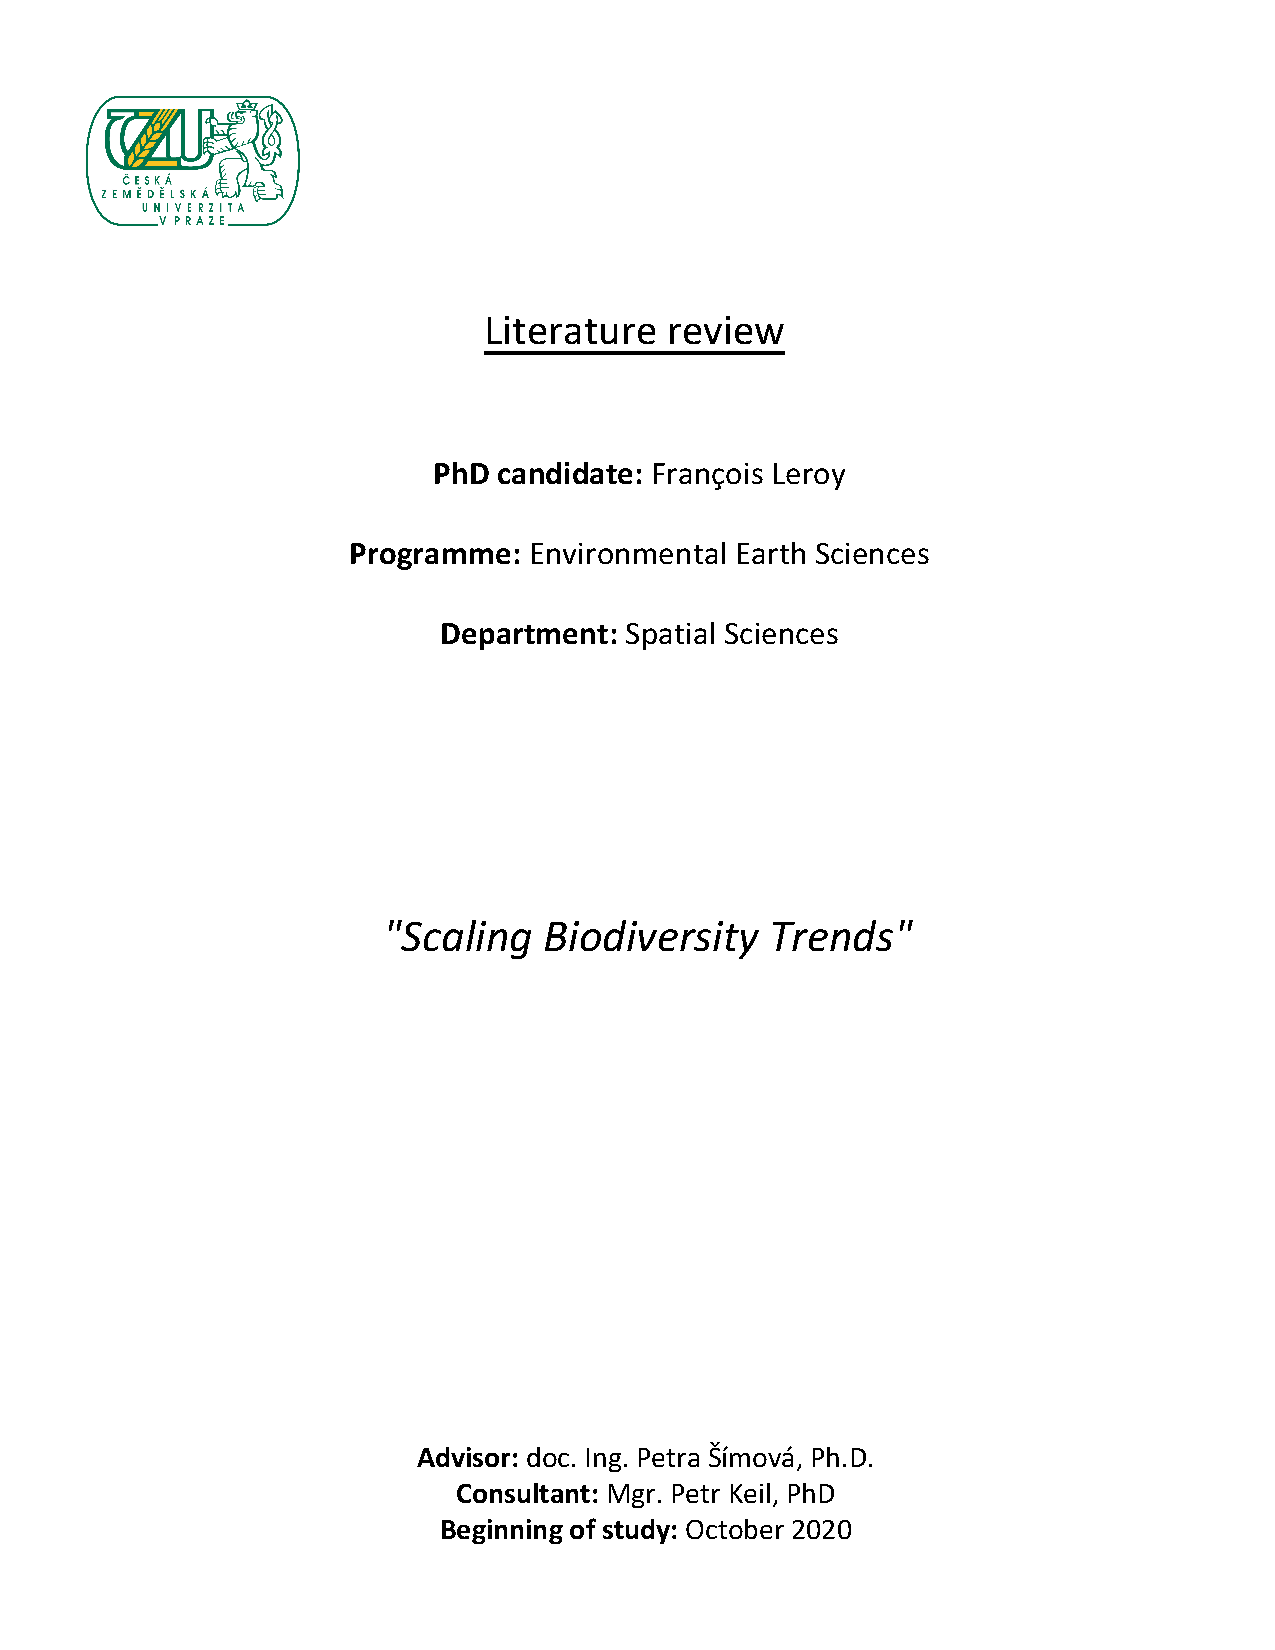
\includepdf[pages = {1}, fitpaper=true]{_assets/coverpage.pdf}

% Roman numbering for content before toc and toc itself
\cleardoublepage 
\pagenumbering{roman}

{
\hypersetup{linkcolor=}
\setcounter{tocdepth}{1}
\tableofcontents
\newpage
}
\vspace{50mm}
\setstretch{1.5}


% Start the arabic numbering at the 1st chapter
\cleardoublepage 
\pagenumbering{arabic}


% The mind, the...
\hypertarget{outline}{%
\chapter*{Outline}\label{outline}}
\addcontentsline{toc}{chapter}{Outline}

Literature review about the link between biodiversity facets trends and spatial/temporal scales.

The idea is to take every paper that talk about biodiversity trends (so far using just the species richness seems already a lot of paper) and to list \textbf{1)} which biodiversity metric they use \textbf{2)} which taxon/taxa they use, \textbf{3)} the spatial scale, \textbf{4)} the temporal scale and \textbf{5)} what is the dynamic (does the biodiversity metric increase/decrease/doesn't change over time/unclear).

Make a table of all these papers and \texttt{group\_by(taxa)\ \%\textgreater{}\%\ order\_by(spatial\_scale\ \textbar{}\ temporal\_scale)}. Then see if for each taxa we can find a trend (a bit like in Chase \emph{et al.} 2019 Oikos paper \textbar{} Jarzyna \emph{et al.} 2015 but here I am not making the analysis, just taking the analysis from papers). Best example found so far: \href{https://besjournals.onlinelibrary.wiley.com/doi/10.1111/j.0021-8901.2004.00926.x}{Hill \& Hamer 2004}

\textbf{Meeting with Petr}

\begin{enumerate}
\def\labelenumi{\arabic{enumi})}
\tightlist
\item
  How is the trend of biodiversity metrics linked to spatial grain/spatial extent and temporal grain/temporal extent.
\end{enumerate}

\begin{itemize}
\item
  Talk about papers which does compare (Jarzyna Jetz)
\item
  The inconsistency of reporting scales (especially for models as in Jiguet et al.or Chiron et al., and for MSI metrics)
\end{itemize}

\begin{enumerate}
\def\labelenumi{\arabic{enumi})}
\setcounter{enumi}{1}
\tightlist
\item
  Data heterogeneity
\end{enumerate}

\begin{itemize}
\item
  Lack of spatial replication. That's why this review is important
\item
  The inconsistency of reporting scales (especially for models, and for MSI metrics)
\item
  Lack in other than western countries
\item
  Metric heterogeneity (Freixedas 2001 but they don't mention the macroecological ones as McGill, my struggle because of the time for space substitution as Hill \& Hammer). Some metrics takes into account temporal dynamic but some papers don't look at the trend of these metrics (Jarzyna et al.~2015)
\item
  Can we use space for time substitution as an actual substitution (Hill \& Hammer)
\item
  Pop trends are usually stronger (cf.~all the abundance metrics)
\end{itemize}

\begin{enumerate}
\def\labelenumi{\arabic{enumi})}
\setcounter{enumi}{2}
\tightlist
\item
  Future directions
\end{enumerate}

\begin{itemize}
\tightlist
\item
  Lack of data for other thsn western cvountries: important to harvest data in other countries
\end{itemize}

\hypertarget{dashboard}{%
\chapter*{Dashboard}\label{dashboard}}
\addcontentsline{toc}{chapter}{Dashboard}

\href{https://www.sciencedirect.com/science/article/pii/S1470160X20306658?via\%3Dihub}{Reference paper}

\begin{itemize}
\item
  05/07/2021: research wos made with the literature review filter for the first query (stopped at \#13) and created the second query (stopped at \#2)
\item
  07/07/2021: questions to Petr: \textbf{1)} can the geometric mean of relative abundance + the weighted goodness of fit be used as biodiversity trend index, \textbf{2)} can the Farmland Bird Indicator (FBI) be used as biodiversity trend (for me it is more biodiversity health, Chiron et al 2013) \textbf{3)} what about the Red List Index trend? \textbf{4)} what about Multispecies population indexes?
\item
  08/07/2021: stopped at the article 41 for research \#2.
\item
  12/08/2021: stopped at article 4 for research \#4
\item
  13/08/2021: stopped at article 8 for research \#4
\item
  17/08/2021: stopped at article 15 for research \#4
\item
  18/08/2021: stopped at article 30 for research \#4
\item
  19/08/2021: stopped at article 46 for research \#4
\item
  20/08/2021: stopped at article 64 for research \#4
\item
  01/09/2021: verifying spatial scales --\textgreater{} stopped at Dittrich 2019
\item
  02/09/2021: \textbf{Question 1:} for the FBI/WBI\ldots*BI indexes, usually they use a GLM/GAM to predict the abundance over the entire spatial extent and then compute the metric. Basically, those metrics are geometric means of predicted species abundances. Which spatial scale to use: the spatial unit of the prediction (i.e.~the plot), or the entire area predicted? (Imo, the second option is correct). \textbf{Question 2:} same question for the Geometric mean but I am realizing while writing this question that *BI are kind of similar to geometric means so answering the first question will answer this one.
\end{itemize}

\textbf{Papers that are driving me mad:} \citet{doxa_low-intensity_2010}, \citet{jiguet_french_2012}, and \citet{chiron_forecasting_2013}, \citet{eglington_disentangling_2012}

\hypertarget{introduction}{%
\chapter{Introduction}\label{introduction}}

Human life quality is intrinsically linked to ecosystems state that he is living in. Indeed, ecosystems services extend in a large spectrum of mechanisms including nutrient cycle, food production, or climate and water cycle regulation \citep{pereira_global_2012}. Some of those ecosystem functions are managed by bird biodiversity such as seed dispersal, controls pests or pollinate plant. Unfortunately, anthropogenic stressors like habitat loss, over exploitation, pollution or introduction of invasive species could lead biodiversity to its sixth mass extinction \citep{barnosky_has_2011}.

Biodiversity erosion is now known from everyone and political decisions has been stated in order to limit it \citep[\emph{e.g.}][2010, 2002]{the_convention_on_biological_diversity_convention_2021}. However, these objectives have been so far not reached due mainly to our confusion and misunderstanding about biodiversity dynamic and how to determine it.

As a matter of fact, studying biodiversity can be confusing, especially because several choices must be done. Firstly, the level at which you are looking at the biodiversity must be chosen (\emph{e.g.} species, functional, phylogenetic diversity). Secondly, one must decide which metric is the most appropriate for his study. There are many facets of biodiversity that can be measured by different metrics depending on the objective of your study. Measures of static biodiversity are commonly used such as species richness or \(\alpha\) diversity \citep[\emph{i.e.} number of species,][]{whittaker_vegetation_1960}, the Shannon index \citep{shannon_mathematical_1948} ,the Simpson index \citep{simpson_measurement_1949} or the Hill number \citep{hill_diversity_1973}. The later three biodiversity indexes take into account the relative abundances of the species and can be considered as the \emph{quality} of the biodiversity. On an other hand, the spatial and temporal \(\beta\) diversity will measure the species turnover and can be measured thanks to Whittaker's \citep{whittaker_evolution_1972}, Sørensen's \citep{sorensen_method_1948} or Jaccard's \citep{jaccard_distribution_1912} dissimilarity indexes \citep[\emph{e.g.}][]{keil_patterns_2012}.

However, overall biodiversity (\emph{i.e.} taking into account species of every taxa) may not be relevant for one's case study. Thus, several multi-species indicators have also been created, taking into account the abundances of indicator species giving information on the ecosystem health. The most known ones are the Red List Index \citep{butchart_improvements_2007, butchart_using_2005, butchart_measuring_2004} or the Biodiversity Change Index \citep{normander_indicator_2012}.

Using all the metrics cited above, we now know that the loss of global biodiversity is unprecedented. However, current scientific literature has also shown that temporal trends in local changes of biodiversity can be opposite to trends at larger scales \citep[\emph{e.g.}][]{chase_species_2019}. Thus, current changes in biodiversity is far more complex than a simple global decrease: most of the ecosystems undergo alterations of their communities with changes in species composition \citep{blowes_geography_2019, dornelas_quantifying_2013}. Wonders persist about how the trend of these different metrics of biodiversity are link to the spatial and temporal scales used when measured.

In order to investigate this link between spatial scales and biodiversity metrics, birds is a relevant taxon. Thanks to the many ornithological monitoring and surveys, we now have a large number of long, high-quality time series on bird populations \citep{bejcek_velke_2016}. Birds are easy to observe, easy to identify and thus many volunteers are motivated to conduct standardized sampling. Given their ability to change quickly of locations, their presence is also a good indicator for ecosystem health and thus several standardized metrics have been created to assess their populations. For instance, the geometric mean of relative abundances or the goodness-of-fit statistic \citep{studeny_goodness_2011} are some of the baseline. Other multi-species indicators have also been created specifically for birds, such as the Farmland Bird Indicator \citep{gregory_developing_2005}, the Forest Bird Indicator \citep{gregory_population_2007} or the Wild Bird Indicator \citep{gregory_wild_2010}.

Here, I propose to review articles assessing the temporal trends of different avian biodiversity metrics and to look at which spatial scales these studies have been done. Summarizing the trends of these qualitative and/or quantitative avian biodiversity indexes along with their spatial and temporal scales will help to see more clearly how the trends of biodiversity are linked to spatio-temporal scales. It is also important to demonstrate that the information about the sampling plan (\emph{i.e.} spatial scale, time span, temporal scales etc) is not systematically indicated in the scientific literature and can bring confusion to the analysis and comparisons of their trends. I believe that this review can help to have a better overview of the current knowledge on the trend of biodiversity metrics of bird populations.

\textcolor{red}{specify that it is mainly for continental/coastal birds but no look at  islandic communities}

\hypertarget{materials-and-methods}{%
\chapter{Materials and Methods}\label{materials-and-methods}}

For this review, articles of interest were the ones assessing temporal trends of the most common indicators (\emph{i.e.} metrics) of avian biodiversity and specifying spatial and temporal scales. For this, I used the \emph{\enquote{advanced search}} tool of the ISI Web of Science Core collection database with these four following queries:

\begin{enumerate}
\def\labelenumi{\arabic{enumi}.}
\item
  \texttt{AB\ =\ ((biodiversity\ OR\ species\ richness\ OR\ diversity)\ AND\ (temporal\ trend*\ OR\ dynamic*)\ AND\ (bird*\ OR\ avia*))} which resulted in 1346 references.
\item
  \texttt{AB\ =\ ((biodiversity\ change\ index)\ \ AND\ (bird*\ \ OR\ avia*)\ \ AND\ trend*)} which resulted in 60 references.
\item
  \texttt{AB\ =\ ((species\ richness)\ AND\ (bird*\ OR\ avia*)\ AND\ trend*)} which resulted in 313 references.
\item
  \texttt{ALL=(birds\ AND\ species\ richness\ AND\ temporal\ trend)} which resulted in 88 references.
\end{enumerate}

For each query, the title and abstract of the articles were reviewed. When the temporal trend was explicitly specified (either visually or literally), the material and method part was read in order to collect the \emph{spatial grain} of the trend (\emph{i.e.} the area at which the trend is assessed), its \emph{temporal grain} (\emph{i.e.} the time span at which data have been gathered on the field), the \emph{spatial extent} (\emph{i.e.} the entire area at which the study applies), the \emph{temporal extent} and the \emph{beginning and ending years} of the study as well as the \emph{general trend} of the metric (Tab. \ref{tab:maintable}).

Concerning the trend assessment, some papers contained the \emph{p-value} or directly specified the significant trend of the metric. However, a portion of papers gives only visual representations of the trend. For those, the standard error was used when displayed. For the very few only giving the trend, \textcolor{red}{the rule of thumb was applied}. Information can be found in the column \emph{Note} of the Tab. \ref{tab:notetable} of the supplementary material. Moreover, the final trend retained (\emph{i.e.} either \emph{Increase}, \emph{Stable} or \emph{Decrease}) doesn't reflect all the fluctuations of the metric through time but rather the difference between the starting and ending points.

Moreover, \citet{pilotto_meta-analysis_2020} conducted a meta-analysis in which they computed and summarized the trend of four biodiversity metrics (namely, species richness, species diversity, abundance and temporal turnover). Some of them were concerning bird communities. For those latter, I used their code and data on the \href{https://github.com/FrsLry/R-code}{github repository} of their paper in order to compute the trends of these four metrics for the bird datasets.

\hypertarget{results}{%
\chapter{Results}\label{results}}

\begin{itemize}
\item
  First of all: there was 9 \emph{Decrease}, 31 \emph{Increase} and 14 \emph{Stable} computed trends across the literature.
\item
  For each metric, the proportion of trend directions are:
\end{itemize}

\begin{tabular}{>{\raggedright\arraybackslash}p{20em}|r|r|r|r}
\hline
rownames & Decrease & Increase & Stable & n\\
\hline
Abundance & 0.3333333 & 0.2666667 & 0.4000000 & 15\\
\hline
Diversity & 0.0000000 & 1.0000000 & 0.0000000 & 2\\
\hline
Evenness & 0.3333333 & 0.6666667 & 0.0000000 & 3\\
\hline
Functional diversity & 1.0000000 & 0.0000000 & 0.0000000 & 1\\
\hline
Functional evenness & 0.0000000 & 1.0000000 & 0.0000000 & 1\\
\hline
Functional richness & 0.0000000 & 1.0000000 & 0.0000000 & 1\\
\hline
Simpson & 0.0000000 & 1.0000000 & 0.0000000 & 2\\
\hline
Spatial beta-diversity & 0.0000000 & 0.0000000 & 1.0000000 & 1\\
\hline
SR & 0.0909091 & 0.6818182 & 0.2272727 & 22\\
\hline
Temporal beta-diversity & 0.0000000 & 0.6666667 & 0.3333333 & 6\\
\hline
\end{tabular}

\begin{landscape}\begingroup\fontsize{10}{12}\selectfont

\begin{longtable}[t]{>{\raggedright\arraybackslash}p{6.5em}>{\raggedright\arraybackslash}p{6.5em}>{\raggedright\arraybackslash}p{6.5em}>{\raggedleft\arraybackslash}p{6.5em}>{\raggedleft\arraybackslash}p{6.5em}>{\raggedleft\arraybackslash}p{6.5em}>{\raggedright\arraybackslash}p{6.5em}>{\raggedright\arraybackslash}p{6.5em}>{\raggedright\arraybackslash}p{6.5em}}
\caption{\label{tab:maintable}Trends of different metrics of biodiversity at various spatial and temporal scales}\\
\toprule
Reference & Metric & Spatial grain (Km²) & Temporal grain (year) & Spatial extent (Km²) & Temporal extent (year) & Years & Country & Trend\\
\midrule
\endfirsthead
\caption[]{\label{tab:maintable}Trends of different metrics of biodiversity at various spatial and temporal scales \textit{(continued)}}\\
\toprule
Reference & Metric & Spatial grain (Km²) & Temporal grain (year) & Spatial extent (Km²) & Temporal extent (year) & Years & Country & Trend\\
\midrule
\endhead

\endfoot
\bottomrule
\endlastfoot
\cellcolor{gray!6}{\cite{harrison_assessing_2014}} & \cellcolor{gray!6}{Abundance} & \cellcolor{gray!6}{10000} & \cellcolor{gray!6}{1.0} & \cellcolor{gray!6}{200000} & \cellcolor{gray!6}{18} & \cellcolor{gray!6}{1994-2011} & \cellcolor{gray!6}{Great Britain, UK} & \cellcolor{gray!6}{Increase}\\
 & Abundance & 10000 & 1.0 & 200000 & 18 & 1994-2011 & Great Britain, UK & \vphantom{1} Stable\\
\cellcolor{gray!6}{} & \cellcolor{gray!6}{Abundance} & \cellcolor{gray!6}{10000} & \cellcolor{gray!6}{1.0} & \cellcolor{gray!6}{200000} & \cellcolor{gray!6}{18} & \cellcolor{gray!6}{1994-2011} & \cellcolor{gray!6}{Great Britain, UK} & \cellcolor{gray!6}{Stable}\\
\cite{pilotto_meta-analysis_2020} & SR & Local & NA & 10180000 & NA & NA & Europe & Increase\\
\cellcolor{gray!6}{} & \cellcolor{gray!6}{Simpson} & \cellcolor{gray!6}{Local} & \cellcolor{gray!6}{NA} & \cellcolor{gray!6}{10180000} & \cellcolor{gray!6}{NA} & \cellcolor{gray!6}{NA} & \cellcolor{gray!6}{Europe} & \cellcolor{gray!6}{Increase}\\
\addlinespace
 & Abundance & Local & NA & 10180000 & NA & NA & Europe & Stable\\
\cellcolor{gray!6}{} & \cellcolor{gray!6}{Temporal beta-diversity} & \cellcolor{gray!6}{Local} & \cellcolor{gray!6}{NA} & \cellcolor{gray!6}{10180000} & \cellcolor{gray!6}{NA} & \cellcolor{gray!6}{NA} & \cellcolor{gray!6}{Europe} & \cellcolor{gray!6}{Stable}\\
\cite{barnagaud_temporal_2017} & SR & 25 & 1.0 & 9834000 & 41 & 1970-2011 & USA & Increase\\
\cellcolor{gray!6}{} & \cellcolor{gray!6}{Evenness} & \cellcolor{gray!6}{25} & \cellcolor{gray!6}{1.0} & \cellcolor{gray!6}{9834000} & \cellcolor{gray!6}{41} & \cellcolor{gray!6}{1970-2011} & \cellcolor{gray!6}{USA} & \cellcolor{gray!6}{Increase}\\
\cite{reif_changes_2013} & SR & 2.5 & 1.0 & 79000 & 23 & 1982-2004 & Czech Rep. & Stable\\
\addlinespace
\cellcolor{gray!6}{} & \cellcolor{gray!6}{SR} & \cellcolor{gray!6}{79000} & \cellcolor{gray!6}{1.0} & \cellcolor{gray!6}{79000} & \cellcolor{gray!6}{23} & \cellcolor{gray!6}{1982-2004} & \cellcolor{gray!6}{Czech Rep.} & \cellcolor{gray!6}{Stable}\\
 & Spatial beta-diversity & 2.5 & 1.0 & 79000 & 23 & 1982-2004 & Czech Rep. & Stable\\
\cellcolor{gray!6}{\cite{schipper_contrasting_2016}} & \cellcolor{gray!6}{Abundance} & \cellcolor{gray!6}{25} & \cellcolor{gray!6}{5.0} & \cellcolor{gray!6}{24710000} & \cellcolor{gray!6}{40} & \cellcolor{gray!6}{1971-2010} & \cellcolor{gray!6}{Canada, USA, Mexico} & \cellcolor{gray!6}{Increase}\\
 & SR & 25 & 5.0 & 24710000 & 40 & 1971-2010 & Canada, USA, Mexico & Increase\\
\cellcolor{gray!6}{} & \cellcolor{gray!6}{Diversity} & \cellcolor{gray!6}{25} & \cellcolor{gray!6}{5.0} & \cellcolor{gray!6}{24710000} & \cellcolor{gray!6}{40} & \cellcolor{gray!6}{1971-2010} & \cellcolor{gray!6}{Canada, USA, Mexico} & \cellcolor{gray!6}{\vphantom{1} Increase}\\
\addlinespace
 & Diversity & 25 & 5.0 & 24710000 & 40 & 1971-2010 & Canada, USA, Mexico & Increase\\
\cellcolor{gray!6}{} & \cellcolor{gray!6}{Functional richness} & \cellcolor{gray!6}{25} & \cellcolor{gray!6}{5.0} & \cellcolor{gray!6}{24710000} & \cellcolor{gray!6}{40} & \cellcolor{gray!6}{1971-2010} & \cellcolor{gray!6}{Canada, USA, Mexico} & \cellcolor{gray!6}{Increase}\\
 & Functional evenness & 25 & 5.0 & 24710000 & 40 & 1971-2010 & Canada, USA, Mexico & Increase\\
\cellcolor{gray!6}{} & \cellcolor{gray!6}{Functional diversity} & \cellcolor{gray!6}{25} & \cellcolor{gray!6}{5.0} & \cellcolor{gray!6}{24710000} & \cellcolor{gray!6}{40} & \cellcolor{gray!6}{1971-2010} & \cellcolor{gray!6}{Canada, USA, Mexico} & \cellcolor{gray!6}{Decrease}\\
\cite{sorte_changes_2005} & SR & 25 & 1.0 & 9834000 & 36 & 1968-2003 & USA & Increase\\
\addlinespace
\cellcolor{gray!6}{} & \cellcolor{gray!6}{Abundance} & \cellcolor{gray!6}{25} & \cellcolor{gray!6}{1.0} & \cellcolor{gray!6}{9834000} & \cellcolor{gray!6}{36} & \cellcolor{gray!6}{1968-2003} & \cellcolor{gray!6}{USA} & \cellcolor{gray!6}{Decrease}\\
 & Evenness & 25 & 1.0 & 9834000 & 36 & - & USA & Decrease\\
\cellcolor{gray!6}{\cite{wretenberg_changes_2010}} & \cellcolor{gray!6}{SR} & \cellcolor{gray!6}{0,03} & \cellcolor{gray!6}{1.0} & \cellcolor{gray!6}{1800} & \cellcolor{gray!6}{11} & \cellcolor{gray!6}{1994-2004} & \cellcolor{gray!6}{Sweden} & \cellcolor{gray!6}{Decrease}\\
\cite{ram_what_2017} & SR & 3,2 & 1.0 & 350000 & 18 & 1998-2015 & Sweden & Increase\\
\cellcolor{gray!6}{} & \cellcolor{gray!6}{Abundance} & \cellcolor{gray!6}{1.6} & \cellcolor{gray!6}{1.0} & \cellcolor{gray!6}{350000} & \cellcolor{gray!6}{18} & \cellcolor{gray!6}{1998-2015} & \cellcolor{gray!6}{Sweden} & \cellcolor{gray!6}{Increase}\\
\addlinespace
\cite{harrison_quantifying_2016} & Abundance & 10000 & 0.5 & NA & 20 & 1994-2013 & UK & Increase\\
\cellcolor{gray!6}{} & \cellcolor{gray!6}{Abundance} & \cellcolor{gray!6}{10000} & \cellcolor{gray!6}{0.5} & \cellcolor{gray!6}{NA} & \cellcolor{gray!6}{20} & \cellcolor{gray!6}{1994-2013} & \cellcolor{gray!6}{UK} & \cellcolor{gray!6}{\vphantom{1} Stable}\\
 & Abundance & 10000 & 0.5 & NA & 20 & 1994-2013 & UK & Stable\\
\cellcolor{gray!6}{\cite{jarzyna_taxonomic_2018}} & \cellcolor{gray!6}{SR} & \cellcolor{gray!6}{2500} & \cellcolor{gray!6}{1.0} & \cellcolor{gray!6}{9834000} & \cellcolor{gray!6}{45} & \cellcolor{gray!6}{1969-2013} & \cellcolor{gray!6}{USA} & \cellcolor{gray!6}{Increase}\\
 & SR & 40000 & 1.0 & 9834000 & 45 & 1969-2013 & USA & Increase\\
\addlinespace
\cellcolor{gray!6}{} & \cellcolor{gray!6}{SR} & \cellcolor{gray!6}{640000} & \cellcolor{gray!6}{1.0} & \cellcolor{gray!6}{9834000} & \cellcolor{gray!6}{45} & \cellcolor{gray!6}{1969-2013} & \cellcolor{gray!6}{USA} & \cellcolor{gray!6}{Increase}\\
 & SR & 9834000 & 1.0 & 9834000 & 45 & 1969-2013 & USA & Increase\\
\cellcolor{gray!6}{} & \cellcolor{gray!6}{SR} & \cellcolor{gray!6}{148940000} & \cellcolor{gray!6}{1.0} & \cellcolor{gray!6}{148940000} & \cellcolor{gray!6}{45} & \cellcolor{gray!6}{1969-2013} & \cellcolor{gray!6}{World} & \cellcolor{gray!6}{Decrease}\\
 & Temporal beta-diversity & 2500 & 1.0 & 9834000 & 45 & 1969-2013 & USA & Increase\\
\cellcolor{gray!6}{} & \cellcolor{gray!6}{Temporal beta-diversity} & \cellcolor{gray!6}{40000} & \cellcolor{gray!6}{1.0} & \cellcolor{gray!6}{9834000} & \cellcolor{gray!6}{45} & \cellcolor{gray!6}{1969-2013} & \cellcolor{gray!6}{USA} & \cellcolor{gray!6}{Increase}\\
\addlinespace
 & Temporal beta-diversity & 640000 & 1.0 & 9834000 & 45 & 1969-2013 & USA & Increase\\
\cellcolor{gray!6}{} & \cellcolor{gray!6}{Temporal beta-diversity} & \cellcolor{gray!6}{9834000} & \cellcolor{gray!6}{1.0} & \cellcolor{gray!6}{9834000} & \cellcolor{gray!6}{45} & \cellcolor{gray!6}{1969-2013} & \cellcolor{gray!6}{USA} & \cellcolor{gray!6}{Increase}\\
 & Temporal beta-diversity & 148940000 & 1.0 & 148940000 & 45 & 1969-2013 & World & Stable\\
\cellcolor{gray!6}{\cite{davey_rise_2012}} & \cellcolor{gray!6}{Simpson} & \cellcolor{gray!6}{1} & \cellcolor{gray!6}{1.0} & \cellcolor{gray!6}{242495} & \cellcolor{gray!6}{13} & \cellcolor{gray!6}{1994-2006} & \cellcolor{gray!6}{UK} & \cellcolor{gray!6}{Increase}\\
 & SR & 1 & 1.0 & 242495 & 13 & 1994-2006 & UK & Increase\\
\addlinespace
\cellcolor{gray!6}{} & \cellcolor{gray!6}{Evenness} & \cellcolor{gray!6}{1} & \cellcolor{gray!6}{1.0} & \cellcolor{gray!6}{242495} & \cellcolor{gray!6}{13} & \cellcolor{gray!6}{1994-2006} & \cellcolor{gray!6}{UK} & \cellcolor{gray!6}{Increase}\\
\cite{chiron_forecasting_2013}\cellcolor{gray!6}{} & \cellcolor{gray!6}{Abundance} & \cellcolor{gray!6}{Admin. unit} & \cellcolor{gray!6}{1.0} & \cellcolor{gray!6}{643801} & \cellcolor{gray!6}{14} & \cellcolor{gray!6}{2007-2020} & \cellcolor{gray!6}{France} & \cellcolor{gray!6}{\vphantom{2} Decrease}\\
 & Abundance & Admin. unit & 1.0 & 643801 & 14 & 2007-2020 & France & \vphantom{1} Decrease\\
\cellcolor{gray!6}{} & \cellcolor{gray!6}{Abundance} & \cellcolor{gray!6}{Admin. unit} & \cellcolor{gray!6}{1.0} & \cellcolor{gray!6}{643801} & \cellcolor{gray!6}{14} & \cellcolor{gray!6}{2007-2020} & \cellcolor{gray!6}{France} & \cellcolor{gray!6}{Decrease}\\
 & Abundance & Admin. unit & 1.0 & 643801 & 14 & 2007-2020 & France & Decrease\\
\addlinespace
\cite{van_turnhout_scale-dependent_2007} & SR & Admin. unit & 4.0 & 41543 & 28 & 1973-2000 & Netherlands & Increase\\
\cellcolor{gray!6}{} & \cellcolor{gray!6}{SR} & \cellcolor{gray!6}{25} & \cellcolor{gray!6}{4.0} & \cellcolor{gray!6}{41543} & \cellcolor{gray!6}{28} & \cellcolor{gray!6}{1973-2000} & \cellcolor{gray!6}{Netherlands} & \cellcolor{gray!6}{Increase}\\
 & SR & 41543 & 4.0 & 41543 & 28 & 1973-2000 & Netherlands & Increase\\
\cellcolor{gray!6}{\cite{chase_species_2019}} & \cellcolor{gray!6}{SR} & \cellcolor{gray!6}{150} & \cellcolor{gray!6}{5.0} & \cellcolor{gray!6}{2800000} & \cellcolor{gray!6}{30} & \cellcolor{gray!6}{1982–2011} & \cellcolor{gray!6}{USA, Canada} & \cellcolor{gray!6}{Stable}\\
 & SR & 400 & 5.0 & 2800000 & 30 & 1982–2011 & USA, Canada & Stable\\
\addlinespace
\cellcolor{gray!6}{} & \cellcolor{gray!6}{SR} & \cellcolor{gray!6}{800} & \cellcolor{gray!6}{5.0} & \cellcolor{gray!6}{2800000} & \cellcolor{gray!6}{30} & \cellcolor{gray!6}{1982–2011} & \cellcolor{gray!6}{USA, Canada} & \cellcolor{gray!6}{Stable}\\
 & SR & 1350 & 5.0 & 2800000 & 30 & 1982–2011 & USA, Canada & Increase\\
\cellcolor{gray!6}{} & \cellcolor{gray!6}{SR} & \cellcolor{gray!6}{11000} & \cellcolor{gray!6}{5.0} & \cellcolor{gray!6}{2800000} & \cellcolor{gray!6}{30} & \cellcolor{gray!6}{1982–2011} & \cellcolor{gray!6}{USA, Canada} & \cellcolor{gray!6}{Increase}\\
\cite{bowler_geographic_2021} & Abundance & National unit & 1.0 & 520475 & 27 & 1990-2016 & Czech Rep., Switzerland, Denmark, Germany & Stable\\*
\end{longtable}
\endgroup{}
\end{landscape}

\hypertarget{supplementary-materials}{%
\chapter*{Supplementary materials}\label{supplementary-materials}}
\addcontentsline{toc}{chapter}{Supplementary materials}

\begin{landscape}\begingroup\fontsize{10}{12}\selectfont

\begin{longtable}[t]{>{\raggedright\arraybackslash}p{6.5em}>{\raggedright\arraybackslash}p{6.5em}>{\raggedright\arraybackslash}p{6.5em}>{\raggedright\arraybackslash}p{40em}}
\caption{\label{tab:notetable}Supplementary informations about each article}\\
\toprule
Reference & Spatial grain (Km²) & Trend & Note\\
\midrule
\endfirsthead
\caption[]{\label{tab:notetable}Supplementary informations about each article \textit{(continued)}}\\
\toprule
Reference & Spatial grain (Km²) & Trend & Note\\
\midrule
\endhead

\endfoot
\bottomrule
\endlastfoot
\cellcolor{gray!6}{\cite{harrison_assessing_2014}} & \cellcolor{gray!6}{10000} & \cellcolor{gray!6}{Increase} & \cellcolor{gray!6}{To assess the metric, they use a GAM to predict the abundance over the entire area of interest (spatial resolution = 1 Km²) and then compute the geometric mean of species abundance = Multi Species Index (as in \cite{studeny_fine-tuning_2013}) from the prediction. Data used to learn the GAM are sampled from plots of 1 Km². Farmland communities}\\
 & 10000 & Stable & Farmland communities, GoF ($\lambda$ = -1) =  weighted towards the rare species\\
\cellcolor{gray!6}{} & \cellcolor{gray!6}{10000} & \cellcolor{gray!6}{Stable} & \cellcolor{gray!6}{Farmland communities, GoF ( $\lambda$ = -2) weighted towards the common species}\\
\cite{pilotto_meta-analysis_2020}\cellcolor{gray!6}{} & \cellcolor{gray!6}{Local} & \cellcolor{gray!6}{Increase} & \cellcolor{gray!6}{"Analyses of the trends in local biodiversity over large spatial scales"}\\
 & Local & Increase & "Analyses of the trends in local biodiversity over large spatial scales"\\
\addlinespace
 & Local & Stable & "Analyses of the trends in local biodiversity over large spatial \vphantom{1} scales"\\
\cellcolor{gray!6}{} & \cellcolor{gray!6}{Local} & \cellcolor{gray!6}{Stable} & \cellcolor{gray!6}{"Analyses of the trends in local biodiversity over large spatial scales"}\\
\cite{barnagaud_temporal_2017} & 25 & Increase & Mean change of SR at the road scales Area of the road = (40/0.8)*(pi*400\^2) with a road of 40 Km with point counts spaced by 0.8 Km and a census radius of 400m\\
\cellcolor{gray!6}{} & \cellcolor{gray!6}{25} & \cellcolor{gray!6}{Increase} & \cellcolor{gray!6}{Not sure that it is at the road scale: "Taxonomic evenness showed a marginal, yet significant, non-linear increase from close to 0.54 in the first decade to 0.56 in the last decade (Table 1), suggesting a light trend towards a more even distribution of species’ abundances among species within local assemblages "}\\
\cite{reif_changes_2013} & 2.5 & Stable & JPSP data, transect scale\\
\addlinespace
\cellcolor{gray!6}{} & \cellcolor{gray!6}{79000} & \cellcolor{gray!6}{Stable} & \cellcolor{gray!6}{JPSP data, national scale}\\
 & 2.5 & Stable & Jaccard index, pairwise comparisions between transects\\
\cellcolor{gray!6}{\cite{schipper_contrasting_2016}} & \cellcolor{gray!6}{25} & \cellcolor{gray!6}{Increase} & \cellcolor{gray!6}{The metric (i.e. geometric mean) is meaned over each road. Area of the road = 50*(pi*400\^2) with 50 census point per road and a census radius of 400m}\\
 & 25 & Increase & \vphantom{2} NA\\
\cellcolor{gray!6}{} & \cellcolor{gray!6}{25} & \cellcolor{gray!6}{Increase} & \cellcolor{gray!6}{Metric = Shannon}\\
\addlinespace
 & 25 & Increase & Metric = Simpson\\
\cellcolor{gray!6}{} & \cellcolor{gray!6}{25} & \cellcolor{gray!6}{Increase} & \cellcolor{gray!6}{\vphantom{1} NA}\\
 & 25 & Increase & NA\\
\cellcolor{gray!6}{} & \cellcolor{gray!6}{25} & \cellcolor{gray!6}{Decrease} & \cellcolor{gray!6}{\vphantom{1} NA}\\
\cite{sorte_changes_2005} & 25 & Increase & The metric is meaned over each road. Area of the road = 50*(pi*400\^2) with 50 census point per road and a census radius of 400m\\
\addlinespace
\cellcolor{gray!6}{} & \cellcolor{gray!6}{25} & \cellcolor{gray!6}{Decrease} & \cellcolor{gray!6}{NA}\\
 & 25 & Decrease & Metric = evenness\\
\cellcolor{gray!6}{\cite{wretenberg_changes_2010}} & \cellcolor{gray!6}{0,03} & \cellcolor{gray!6}{Decrease} & \cellcolor{gray!6}{looking at the trend through different environmental policies, " local species richness (i.e. at the scale of sites = 3 hectares) decreased significantly probably as a result of an overall reduced abundance of several species. "}\\
\cite{ram_what_2017} & 3,2 & Increase & SR for forest species meaned over roads, spatial grain = 8* .4 with road of 8 Km and census radius no limitations so assumed 200m\\
\cellcolor{gray!6}{} & \cellcolor{gray!6}{1.6} & \cellcolor{gray!6}{Increase} & \cellcolor{gray!6}{MSI for forest species, road of 8 Km with no limitations so assumed 200m}\\
\addlinespace
\cite{harrison_quantifying_2016} & 10000 & Increase & Geomteric mean of species abundance, they predict the abundance with resolution of 1 Km² and then computed the metric for each 10000 Km² cell across Great Britain, Visited twice a year\\
\cellcolor{gray!6}{} & \cellcolor{gray!6}{10000} & \cellcolor{gray!6}{Stable} & \cellcolor{gray!6}{GoF ( $\lambda$ = -1) = toward rare species" The goodness-of-fit-based measure of biodiversity suggests that both rare and common species made gains through much of Britain in the first half of the time period, and losses in the second half.", Visited twice a year / Increase first half and second second halfGoF ( $\lambda$ = -1)}\\
 & 10000 & Stable & GoF ( $\lambda$ = -2) = toward common species " The goodness-of-fit-based measure of biodiversity suggests that both rare and common species made gains through much of Britain in the first half of the time period, and losses in the second half.", Visited twice a year / Increase first half and second second half\\
\cellcolor{gray!6}{\cite{jarzyna_taxonomic_2018}} & \cellcolor{gray!6}{2500} & \cellcolor{gray!6}{Increase} & \cellcolor{gray!6}{NA}\\
 & 40000 & Increase & \vphantom{1} NA\\
\addlinespace
\cellcolor{gray!6}{} & \cellcolor{gray!6}{640000} & \cellcolor{gray!6}{Increase} & \cellcolor{gray!6}{\vphantom{1} NA}\\
 & 9834000 & Increase & \vphantom{1} NA\\
\cellcolor{gray!6}{} & \cellcolor{gray!6}{148940000} & \cellcolor{gray!6}{Decrease} & \cellcolor{gray!6}{NA}\\
 & 2500 & Increase & NA\\
\cellcolor{gray!6}{} & \cellcolor{gray!6}{40000} & \cellcolor{gray!6}{Increase} & \cellcolor{gray!6}{NA}\\
\addlinespace
 & 640000 & Increase & NA\\
\cellcolor{gray!6}{} & \cellcolor{gray!6}{9834000} & \cellcolor{gray!6}{Increase} & \cellcolor{gray!6}{NA}\\
 & 148940000 & Stable & NA\\
\cellcolor{gray!6}{\cite{davey_rise_2012}} & \cellcolor{gray!6}{1} & \cellcolor{gray!6}{Increase} & \cellcolor{gray!6}{They predict the metric using a GAM with spatial resolution of 1 Km². Then they show the trend for the mean value of the metric per year}\\
 & 1 & Increase & \vphantom{1} NA\\
\addlinespace
\cellcolor{gray!6}{} & \cellcolor{gray!6}{1} & \cellcolor{gray!6}{Increase} & \cellcolor{gray!6}{NA}\\
\cite{chiron_forecasting_2013} & Admin. unit & Decrease & Concerning the spatial scale, predictions are made using the spatial unit of 4 Km² and the FBI is computed for each region of France, then meanned. Prediction with baseline scenario\\
\cellcolor{gray!6}{} & \cellcolor{gray!6}{Admin. unit} & \cellcolor{gray!6}{Decrease} & \cellcolor{gray!6}{FBI prediction with CAP greening cenario}\\
 & Admin. unit & Decrease & FBI prediction with No Pillar I scenario\\
\cellcolor{gray!6}{} & \cellcolor{gray!6}{Admin. unit} & \cellcolor{gray!6}{Decrease} & \cellcolor{gray!6}{FBI prediction with biofuel scenario}\\
\addlinespace
\cite{van_turnhout_scale-dependent_2007} & Admin. unit & Increase & For each region, the trend is computed\\
\cellcolor{gray!6}{} & \cellcolor{gray!6}{25} & \cellcolor{gray!6}{Increase} & \cellcolor{gray!6}{Mainly increase of SR but the proportion of negative trend were higher than for the regional scale}\\
 & 41543 & Increase & National scale\\
\cellcolor{gray!6}{\cite{chase_species_2019}} & \cellcolor{gray!6}{150} & \cellcolor{gray!6}{Stable} & \cellcolor{gray!6}{NA}\\
 & 400 & Stable & NA\\
\addlinespace
\cellcolor{gray!6}{} & \cellcolor{gray!6}{800} & \cellcolor{gray!6}{Stable} & \cellcolor{gray!6}{NA}\\
 & 1350 & Increase & NA\\
\cellcolor{gray!6}{} & \cellcolor{gray!6}{11000} & \cellcolor{gray!6}{Increase} & \cellcolor{gray!6}{NA}\\
\cite{bowler_geographic_2021} & National unit & Stable & Metric = MSI, as many and as intense increase (i.e. Czech Rep. and Switzerland) than decrease (i.e. Germany and Denmarl)\\*
\end{longtable}
\endgroup{}
\end{landscape}

\singlespacing


\renewcommand\bibname{References}
  \bibliography{references.bib}

\end{document}
